\documentclass{article}
\usepackage{graphicx,fancyhdr,amsmath,amssymb,amsthm,subfig,url,hyperref,epigraph,lipsum}
\usepackage[margin=1in]{geometry}
\setlength\epigraphwidth{.8\textwidth}

% Bibliography
\usepackage[backend=biber, style=authortitle-comp, refsection=section]{biblatex}
\addbibresource{report.bib}

%----------------------- Macros and Definitions --------------------------

\renewcommand{\theenumi}{\bf \Alph{enumi}}

\fancypagestyle{plain}{}
\pagestyle{fancy}
\fancyhf{}
\fancyhead[RO,LE]{\sffamily\bfseries\large University of Delhi}
\fancyhead[LO,RE]{\sffamily\bfseries\large MCS-204 Advanced Computer Networks}
\fancyfoot[RO,LE]{\sffamily\bfseries\thepage}
\renewcommand{\headrulewidth}{1pt}
\renewcommand{\footrulewidth}{1pt}

\graphicspath{{figures/}}

%-------------------------------- Title ----------------------------------

\title{Emerging Trends in Mobile Communications}
\author{
    Samyak Ahuja \\
    \texttt{Class ID: 29}
    \and
    Mayank Kharbanda \\
    \texttt{Class ID: 16}
}

%--------------------------------- Text ----------------------------------

\begin{document}
\maketitle

\section{Acoustic data transmission}
\epigraph{ I tried to discover, in the rumor of forests and waves, words
that other men could not hear, and I pricked up my ears to listen to the
revelation of their harmony.}{\textcite{november05}}

\subsection{Introduction}
The rise of IoT devices in the home and workplace has created a world where
data and connectivity are becoming increasingly complex. \textcite{ihs16}
predicts a staggering 75 billion connected devices by 2025, up from 26 billion
in 2019, as shown in Figure \ref{fig:ihs_iot}.  As IoT technology advances and the
demand for efficient ways of communicating data between these devices grows,
the world has witnessed a rise in emerging new data transmission technologies
which are looking to provide secure and effective solutions for sharing
information. One solution rising to meet these new demands is “data-over-sound”.

\begin{figure}[!h]
  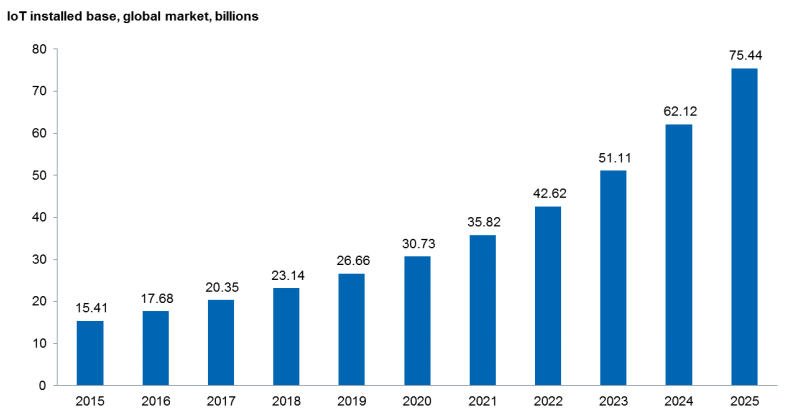
\includegraphics[width=\linewidth]{res/iot_market_trend.png}
    \caption{Number of IOT devices that will be installed worldwide from 2019
    to 2025 (in billions).}
  \label{fig:ihs_iot}
\end{figure}


Data-over-sound (DoS) presents a compelling solution for many device-to-device
connectivity applications, particularly for use cases that require
frictionless, low cost connectivity with nearby devices. DoS harnesses devices’
existing speakers and microphones to send and receive data over an acoustic
channel. Because it doesn’t require any additional networking hardware, DoS has
captured the interest of companies interested in adding wireless connectivity
functionality to existing devices. Some big names such as Google and Cisco
already have point-product DoS integrations

There are a number of connectivity technologies available in the market today,
including extremely short range (NFC and QR); short range, high bandwidth
(Bluetooth and Wi-Fi). Each technology has its advantages which makes it more
or less suitable for certain applications. An overview of these considerations
are given in Table \ref{table:feature_dos}.

\begin{table}[!h]
\begin{center}
\begin{tabular}{r|c|c|c|c|c|c|}
\multicolumn{1}{r}{}
 &  \multicolumn{1}{c}{DoS}
 &  \multicolumn{1}{c}{QR}
 &  \multicolumn{1}{c}{NFC}
 &  \multicolumn{1}{c}{Bluetooth}
 &  \multicolumn{1}{c}{Wi-Fi}
 &  \multicolumn{1}{c}{Li-Fi} \\
\cline{2-7}
    Two-way communication & 1 & 0 & 0 & 1 & 1 & 1 \\
\cline{2-7}
    One-to-many broadcast & 1 & 0 & 0 & 0 & 0 & 1 \\ 
\cline{2-7}
    Non line-of-sight communication & 1 & 0 & 0 & 1 & 1 & 0 \\
\cline{2-7}
    Zero pairing/set-up procedure & 1 & 1 & 1 & 0 & 0 & 0 \\
\cline{2-7}
    Low power operation & 1 & 1 & 1 & 1 & 0 & 0 \\
\cline{2-7}
    max data rate & 1 kb/s & 3 kb & 424 kb/s & 25 mb/s & 70 mb/s & 1 gb/s \\
\cline{2-7}
    max range & 100m & 10:1 & 20/cm & 100/cm & 50m & 10m \\
\cline{2-7}
\end{tabular}
\end{center}
\caption{Feature comparison for DoS vs alternative technologies}
\label{table:feature_dos}
\end{table}

\subsection{Advantages of Data-over-Sound}

According to Table \ref{table:feature_dos} following advantages can be listed.

\begin{description}
    \item [Device interoperability] The simple hardware requirement of a
        speaker and/ or microphone make data-over-sound arguably the most
        wide-reaching wireless communication technology in terms of device
        compatibility. Mobile phones, voice controlled devices, and any device
        with an alarm speaker are able to communicate using data-over-sound.
        This includes many legacy devices. Data can also be transmitted over
        media channels such as radio and TV, and over existing telephone lines.

    \item [Frictionless UX]  Data-over-sound requires no pairing or
        configuration, making data transfer as simple as pressing a button. 

    \item [Physically Bounded]  Because sound waves respect room boundaries,
        particularly in the near-ultrasonic range commonly used in
        data-over-sound, transmissions do not pass between neighbouring rooms.
        This means that it can be used for detecting the presence of a device
        with room-level granularity.

    \item [Zero power] The advent of ‘wake-on-sound’ MEMs microphones such as
        the Vesper VM1010 enables devices to communicate using data-over-sound,
        whilst draining virtually no battery power in between communications ($<$
        10 µA). 
\end{description}

\printbibliography[heading=subbibliography]


\vspace{2in}
\section{test}
IGNORE IT. This is a test section to see how final document will look when merged. \\

\lipsum[1-1]
\printbibliography[heading=subbibliography]

\end{document}
